\section{Introduction}
Bug localization is one of the important steps in software maintenance.
Especially in issue triaging, where triager has to predict the potential defected components based on his understanding to the issue and the system, then he needs to assign the issue to the right developer who has the required knowledge to fix it.
Automating this step helps speed up bugs fixing and reduce costs in issue triaging.
Lam \etal\cite{lam2017bug} proposed the state of the art approach to automate bug localization by ensemble revised Vector Space Model(rVSM)\cite{zhou2012should} and Deep Neural Network(DNN).  
Similar as most of the existed algorithms, this approach require source code information which is not always available to triagers or the QA team in large companies with code security requirement.
Analyzing the code base dramatically increase the learning time of this kind of algorithm in large projects.
%Moreover, the fast evolution of source code further penalizes this approach that the predictive model has to be updated frequently.   
In this paper, we explore the possibility to predict defected components solely based on information learned from bug reports.

Recurrent neural network(RNN) has been proved to be efficient in capturing semantic as well as syntactic information from text to build statistical language models.
But for source code, Hellendoorn \etal show that the RNN is not better than traditional IR method in language model building\cite{hellendoorn2017deep}.
Bug report is different from common text and source code in that it is generally composed by common text and source code segment or error trace message. 
%We believe that IR method and RNN can learn different information from bug reports and could complement each other.
In this work we want to find out whether deep Recurrent Neural Network can learn from bug report more efficiently than IR based method, namely the Vector Space Model. 
Thus the ensemble of these two could offer better performance than using only one of them.

The contribution of this paper is in two folds:  
\begin{itemize}
	%\item an ensemble of naive tf-idf based VSM and Gated Recurrent Network to recommend high risk components solely based on bug reports.
	\item an naive tf-idf based VSM method and a deep Gated Recurrent Unit Network to recommend high risk components solely based on bug reports.
	%\item By analyzing the performence of the naive tf-idf based VSM and Gated Recurrent Network,  we show that IR method and RNN can learn different information from bug reports and could complement each other to offer better performance in the ensemble method.
	\item By analyzing the performence of the naive tf-idf based VSM and Gated Recurrent Network,  we show that deep Recurrent Neural network achieves 163\% more bug hit by top-k recommendation, 2 times higher Mean Reciprocal Rank(MRR) and 3 times higher Mean Average Precision(MAP) and hence confirm the hypethesis that DRNN can learn better from bug reports.
	\end{itemize}

The paper is organized as the following: 

\section{Background}
\subsection{Bug Localization In Post-release Software Quality Insurrance}
One of the main purpose of software engineering is to deliver high quality product to cients.
However, as software architecture getting more and more complex, the possibility of introducing bugs in the development being higher and higher.  
Different approaches are adopted in the industry to reduce the risk of delivering defeted product, test driven development, unit testing, test regression, peer review etc.
But there are still bugs found by the client after release. 
In this case, being able to fastly locate the defeted components and hence assign the rigth developer to fix the customer reported bugs is critical to post-release software quality insurrance. 

The traditional way is to do the assigning based on the triager's experience and his understanding of the reported issue. 
For experienced triager, they could spot light some potential defected location very fast and accurate.
But for triager with less experience or even new to the project, the process could take longer time and the prediction would not be correct.
Thus they may assign a wrong developer for the issue and reassigning would be required and a longer time to get the bug fixed. 
Jeon \etal \cite{jeong2009improving} reported that the Eclipse project takes on average 40 days for bug assignment and another 100 days for reassigning..
The numbers for Mozilla are 180 days for the first assigning and another 250 days for reassigning.

To help address this problem, recent research applies NLP techniques to learn from bug reports and suggest a ranked list of potential defect location\cite{gay2009use}\cite{lam2017bug}\cite{nguyen2011topic}\cite{zhou2012should}\cite{saha2013improving}\cite{shokripour2013so}, or to suggest the developer who could fix the bug\cite{anvik2011reducing}\cite{bhattacharya2010fine}\cite{xuan2012developer}\cite{jonsson2016automated}.
All these approaches focus on combining source code and code change history from version controling tools(ex: Git)  with bug reports to make the prediction.
However, in companies that has a strict source code security policy, which is a common situation for large companies, source code or even code change history is not available for triagers. 
Bug report is the only source of information they can use to perform the triaging.   
Therefore, in this work we focus on bug localization with only bug reports as the input source.


\subsection{Data Mining Bug Reports}
The most popular technique used in information retrieval from bug reports is the VSM with TF-IDF as entry value\cite{gay2009use}\cite{zhou2012should}. 
Another frequent used algorithm is the Latent Dirichlet Allocation(LDA)\cite{nguyen2011topic}.
And resent works try to ensemble IR techniques with Machine Learning to achieve better performance\cite{jonsson2016automated}\cite{lam2017bug}.
Jonsson \etal \cite{jonsson2016automated} ensemble TF-IDF with different ML algorithms with Stacked Generalization. 
Lam \etal\ \cite{lam2017bug}combines rVSM with DNN.

To the best of our knowledge, there is not past work to use DNN, more specifically deep Recurrent Neural Network independently to learn from bug reports and suggest potential defect location.
In this work, we apply DNN with multiple layers of Gated Recurrent Unit to learning from bug reports, and compare its performance to VSM.
Moreover, we ensemble the DNN with VSM to leverage the performance.

\section{Methodology}

\subsection{Vector Space Model}
Vector Space Model was first proposed by Salton \etal\cite{salton1975vector} to quantify documents.
With a pre-defined and indexed vocabulary of size $s$: $V = \{t_1, t_2,...,t_s\}$, 
each term $t_i$ in a given document $d$ could be represented by a weight quantity $w_i$, where $i$ is its index in the vocabulary $V$.
Thus the given document $d$ could be represented by a vector $d=[w_1,w_2,...,w_s]$.
Obviously, the length of the vector $d$ is the same as the size of the vocabulary.
If a term $t_j$ is not in document $d$, then $w_j = 0$.   
With this vector representation, we can analyze the documents with quantitative methods.

\subsection{TF-IDF}
The selection of weighting method to use in VSM is important to the performance. 
We choose TF-IDF\cite{salton1988term} because of its well reported performance in previous works.
TF is short for term frequency. 
There are different schemes to evaluate TF, in our implementation, we calcuate TF by fomular 1

\begin{equation}
	tf(t,d) = f_{t,d}
\end{equation}

where $t$ is the given term, $d$ is the document and $f_{t,d}$ is the count of term $t$ in document $d$.

IDF is short for Inverse Document Frequency and is generated from equation 2in our implementation.

\begin{equation}
	idf(t) = log\frac{n_d}{df(d,t)} +1
\end{equation}
where $n_d$ is the total of documents and $df(d,t)$ is the number of documents containing term $t$.

Then the weight $w_t$ is given by:
\begin{equation}
	w_t = tf(t)*idf(t)
\end{equation}
 
Then the resulting vector $w$ is normalized to get the vector $d$:
\begin{equation}
	d = \frac{w}{||w||_2} = \frac{w}{\sqrt{\sum_{i=1}^{s}w_i^2}}
\end{equation} 


\subsection{Our VSM Bug Localization Model}
Similar as how to rank risky files based on similar bugs in rVSM\cite{zhou2012should},
after we obtain the vector representation of all bug reports, for a new comming report $d_n$ and an old bug report $d_i$ that has been fixed in the training set $D$ , we calculate their Cosine similarity:
\begin{equation}
	similarity(d_n,d_i) = \frac{d_n \cdot d_i}{||d_n||*||d_i||}
\end{equation}

For a given component $c$, define $D_c$ to be the set of bugs that are fixed by changing code in $c$,  then the risk of $c$ is given by:
\begin{equation}
	risk(c) = min(similarity(d_n,d_i)) \forall d_i \in D_c
\end{equation}

And the components are ranked by their risk score from maximum to minimum.
Our VSM model achieve a MRR of 43.12\%, 19.45\%, 14.40\% and 2.38\%, and a MAP of 39.27\%, 10.73\%, 5.74\% and 1.18\%  for projects ZXing, SWT,AspecJ and Eclipse respectively. 





\subsection{Deep Gated Recurrent Unit Network}
Recurrent Neural Network(RNN) is good at modeling sequential data. 
As Mikolov introduced RNN to language modeling\cite{mikolov2010recurrent}, more and more applications of RNN in document analysis related task are proposed, for example, machine translation. 
In recent years, people starts to apply RNN to model source code\cite{raychev2014code}. 
It is believed that RNN can learn syntactic and semantic rules from text documents.
Given that bug reports are also written by human natural language, we believe that we can use RNN to learn from bug reports and make precise predictions on risky components.
We apply Gated Recurrent Unit in our RNN implementation.
GRU is proposed to solve the gradient vanishing problem in training a (RNN)\cite{chung2014empirical}.
It acheive the same performance as Long Short Term Memory but with less computations.
Its stucture is show in figure \ref{gru}. $h$ is the current state and $\hat{h}$ is context state which could memorize the impact of the input history. 
The reset gate $r$ controls whether the state from the current input should be memorized in $\hat{h}$.
The update gate $z$ controls whether the memory from $\hat{h}$ should considered when updating $h$ to give out prediction.  
\begin{figure}
	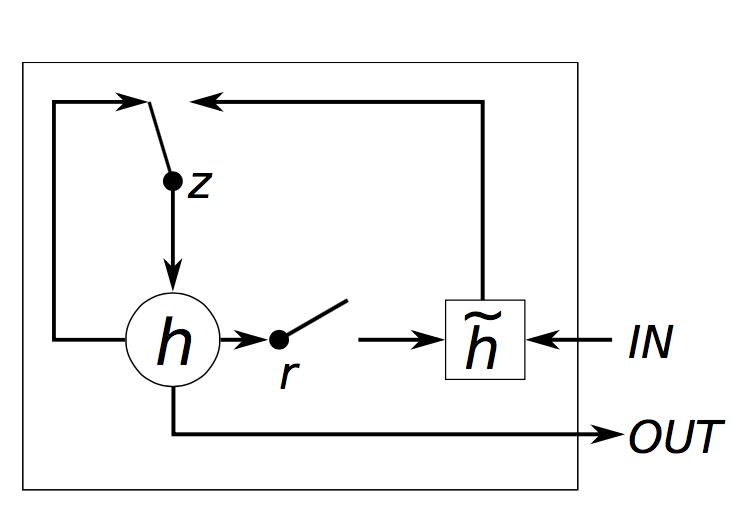
\includegraphics[scale=0.5]{gru.png}
	\caption{Gated Recurrent Unit\cite{chung2014empirical}}
	\label{gru}
\end{figure}

Given the input vector $x_t$ at step t, each gates and states are calcuated recursively as:
\begin{equation}
	z_t = \sigma_g(W_zx_t+U_{z}h_{t-1}+b_z)
\end{equation}	
\begin{equation}
	r_t =  \sigma_g(W_rx_t+U_{r}h_{t-1}+b_r)
\end{equation}	
\begin{equation}
	h_t=(1-z_t) \circ h_{t-1} + z_t \circ \sigma_h(W_hx_t+U_{h}(r_t \circ h_{t-1})+b_h)
\end{equation}
Where $o$ is point-wise multiplication, $W$ and $U$ is the weight matrices for the corresponding component, $b$ is the bias vector.
$\sigma_g$ is the sigmoid activation function which has the form:
\begin{equation}
	\sigma_g(x) = \frac{1}{1+e^{-1}}
\end{equation}
and $\sigma_h$ is the hyperbolic tangent activation function with the form:
\begin{equation}
\sigma_h(x)=\frac{e^x - e^{-x}}{e^x + e^{-x}}	
\end{equation}

In our DRNN implementation, the input layer pass the input vector to the embedding layer which generates the :word embedding of size $100$.
The resulted embedding will then be passed to the stacked hidden GRU layers of size $10$ with each GRU cell of size $100$.
The encoding of the GRU hidden layers is pass to fit a logistic regression to predict the possibility of each components to be defected.
Figure \ref{dnn} illustrates the structure described above. All settings are selected by random withno specific reason.

\begin{figure}
	\includegraphics[scale=0.35]{deep_structure.png}
	\caption{Deep GRU network structure}
	\label{dnn}
\end{figure}

The number of layers and the embedding size is selected randomly. 
Increasing the number of layers could improve performance a litter with longer training time as penalty.
Small change to the embedding size does not change the result siginicantly
Large change (ex: doubling the embedding size) would result in huge memory requirement and failed in runtime.
Our DRNN model achieve a MRR of 34.16\%, 67.92\%, 44.10\% and 11.81\%, and a MAP of 30.83\%, 51.13\%, 21.39\% and 6.53\%  for projects ZXing, SWT,AspecJ and Eclipse respectively. 

%
%\subsection{Ensemble of VSM and GRU}
%Ensemble method \cite{dietterich2000ensemble} is used to combine predictions from multiple different model to give out better performance than a single model.	
%\cite{lam2017bug} ,\cite{wang2014version} and \cite{jonsson2016automated} apply ensemble method to perform bug triage and achieve good performance. 
%Different schemes can be used in ensembling. 
%Stacked Generalization\cite{wolpert1992stacked} is theorectally the most effective one which adds one more classifier to take predictions from ensembled models as input and is trained to reduce prediction error.  
%Jonsson \etal \cite{jonsson2016automated} ensembled TF-IDF with different ML algorithms with Stacked Generalization.
%However, as a preliminary research, we apply a simlper scheme 
%For a given component, we takes the minimum of the two risks given by the two aforemention models as the final risk.
%
%\begin{equation}
%risk(c) = min(risk_{VSM}(c) , risk_{DNN}(c) )
%\end{equation}
%
%\todo {report performace}


 
\section{Experiment Design}

\subsection{Data Set }
We perform our experiment on the exact same data set used in \cite{wang2014version} ,\cite{saha2013improving} and \cite{zhou2012should}.
The detail of the data set is summarized in table \ref{data_table} 


There are in total 3,379 bug reports from four popular open source projects in this data set, AspectJ, Eclipse, SWT, and ZXing. 
\begin{itemize}
	\item ZXing, a barcode image processing library for Android platform, is the smallest data set.
	It contains 20 bugs fixed between March and September 2010 with 391 source files being changed.
	\item SWT is an open source widget tookit. 
	This data set has 98 bugs fixed from October 2004 to April 2010 with 484 source files being fixed. 
	\item AspecJ, An aspect-oriented extension to the Java programming language 
	\item Eclipse, the famous open source integrated development environment, contains 3075 bugs fixed in the period between October 2004 and March 2011 with 12863 files being changed.
\end{itemize}





For each bug report, we can obtain its title, description from the issue reporter, and the files being changed to fixed the reported bug. 

Differently from previous work, the granularity of our experiment is on component level instead of on file level. 
Because we don't use the source code information to simulate a situation of strict source code security, new added files cannot be captured in the prediction with either VSM or DNN.
Thus we first truncate the path of a given file by removing the file name to obtain the component containing the given file. 
We assume that by knowing the potential defected component is enough for assigning the appropriate developer to solve the issue.
Because if a developer knows a component very well, he should also has knowledge to the new added file to that component.
After the truncation, there are 11, 15, 555 and 534 components in ZXing , SWT, Eclipse and AspectJ respectively. 
We removed one bug from the SWT project since the defected file has no component level, it locates in the top most directory. 
Removing one record does not impact on the performance evaluation given the relatively large number of bugs. 
The detail of the three data sets is summarized in table \ref{data_table}

\subsection{Preprocessing}
Bug reports is different from normal text in that it could has code elements, source file names or error log in its content. 
Here we list some examples to illustrate the situation. 
This is some bug description from the Eclipse project:

\textbf{Bug 77046:}If the Pattern Match job is already running when the console's partitioner reports that it is finished work, it is possible that the pattern matcher can think that it's finished before checking the entire document. This is the trace from the failed test: Incorrect number of messages logged for build. Should be 8. Was 2 junit.framework.AssertionFailedError: Incorrect number of messages logged for build. Should be 8. Was 2 at\\ org.eclipse.ant.tests.ui.BuildTests.testOutput(BuildTests.java:41) at\\ sun.reflect.NativeMethodAccessorImpl.invoke0(Native Method) at\\ sun.reflect.NativeMethodAccessorImpl.invoke\\(NativeMethodAccessorImpl.java:39) at\\ sun.reflect.DelegatingMethodAccessorImpl\\.invoke(DelegatingMethodAccessorImpl.java:25) at\\ org.eclipse.ant.tests.ui.AbstractAntUIBuildTest.access\$0\\(AbstractAntUIBuildTest.java:1) at\\ org.eclipse.ant.tests.ui.AbstractAntUIBuildTest\$1\\.run(AbstractAntUIBuildTest.java:44) at\\ java.lang.Thread.run(Thread.java:534)



After the normal text describing the issue, the reporter also attached the error trace log as well.
If we don't perform the preprocessing correctly, neither VSM or DRNN model could learn patterns from the error trace log, since the long component name would be seen as one term, but actually there are multiple important terms there. 
For example, the path\\ "org.eclipse.ant.tests.ui.BuildTests.testOutput(BuildTests.java:41)"\\ contains important terms: ui,Build,Test. Here is another example:

\textbf{Bug 76208}
Boolean.getBoolean((String)newValue) queries if a system property exists with the argument name...not what we want in this context.


The reporter is reporting an undesired functionality from a code segment. Again important terms would be missed if we don't separate the code segment correctly. 

Thus we replace all non word character by white space to separate terms, and if a small case character followed by an upper case character, the separate them by a white space. 
We also remove all numbers to reduce the size of the vocabulary and hence the requirement on computation resource. 
After the preprocessing, we summarize the data set detail in table \ref{data_table}.We apply the 80-20\% split to generate the training and testing set for each project.

\begin{table*}[!tbh]
	\begin{center}
		\caption{Data Set Summary}
		\label{data_table}
		
		\begin{tabular}{c|l|l|l|l|l} %
			\textbf{Project} & \textbf{Description} & \textbf{\#bugs} & \textbf{period} & \textbf{\#files} & \textbf{\#component}\\
			\hline\hline
			ZXing & barcode image processing  & 20 & 2010.3-& 391 &11\\
                  &library  for Android platform & &  2010.10 & & \\			
			SWT & open source widget & 98 & 2004.10-& 484 &15\\
			v3.1 &  tookit & &2010.4 & &\\
			AspecJ & An aspect-oriented  & 286 &2002.6 & 6485 & 534\\
			       &   extension to the Java & & -2006.10 & &\\
			       &    programming language & & & &\\
			Eclipse & open source integrated& 3075&2004.10- & 12863& 555\\
 			 v3.1 &  development environment& &2011.3 &  &\\
		\end{tabular}
	\end{center}
\end{table*}

\subsection{Metrics}
To evaluate the performance of different models, we apply the following common used metrics:

\textbf{Top-k Bugs Hit}
Top-k bugs hit is the number of bugs that are correctly localized from the top k components in the output ranked list. 
At least one component has to been captured in the top k list for the given prediction be classified as a hit.

\textbf{Mean Reciprocal Rank(MRR)} is a measure to evaluate the quality of the ranked list from a recommendation system. 
If for all queries under test, the higer the the first hit relevant item is ranked, the higher value the MRR will be and vice versus. 
It's calculated by the following formula:
\begin{equation}
MRR = \frac{1}{|Q|}\sum^{i \in Q}\frac{1}{rank_i}
\end{equation} 
Where $Q$ is the set of test queries, in our context would be the bugs in the testing data set. 
$i$ is a particular bug in $Q$ and $rank_i$ is the ranking of the first collect prediction in the output list.

MRR only cares about the ranking of the first correct prediction. 
However, there could be multiple defected components for one reported bug. 
We also need to check how well different models rank the other defected components.

\textbf{Mean Average Precision(MAP)} To evaluate how well different models rank all defected components we first calculate the average precision for one bug report:
 \begin{equation}
 	AP=\frac{1}{|C|} \sum_{i=1}^{N}prec(i)*relevance(i)
 \end{equation}
Where $C$ is the set of all defected components for the given bug. 
$N$ is the total number of components in the system.  
$prec(i)$ is the precision for the top-i list.
$relevance(i)$ is 1 if the $i^{th}$ item is defected, otherwise $0$.

Then MAP is calculated by the equation:
\begin{equation}
	MAP = \frac{1}{|Q|}\sum^{Q_i \in Q}AP(Q_i)
\end{equation} 

The model with higher MAP score is the better.
\section{Evaluation and Discussion}

\subsection{Experiment Result}

We report the performance of the three models in table \ref{performance_top_k}, \ref{performance_MRR} and \ref{performance_map}.
For the project Zxing and SWT, because the total of  their components is close to 10, we report the top-1 bug hit rate.
For the project AspectJ and Eclipse, given the large  number of components, we report the top-10 bug hit rate.

As shown in Table \ref{performance_top_k}, All models acheive 100\%  bug hit for the project ZXing, DRNN achieves the best result in all other three projects. It gets 100\%, 79.31\% and 20.29\% hit rate for the project SWT, AspectJ and Eclipse respectively. 
VSM achieves the lowest bug hit rate which is 50\%, 41.38\% and 3.6\% for SWT, AspectJ and Eclipse respectively. 
DRNN achieve 163.82\% more bugs hit on average than VSM.

 \begin{table}[h]
 	\begin{center}
 		\caption{Top k bugs hit}
 		\label{performance_top_k}
 		
 		\begin{tabular}{c|l|l} %
 			 \textbf{Projects} & \textbf{VSM} & \textbf{DRNN}\\
 			\hline\hline
 			ZXing(top-1)& 4(100\%)&4(100\%)  \\
 			
 			SWT(top-1) & 10(50\%) & \textbf{20(100\%)} \\
 			
 			AspecJ(top-10) & 24(41.38\%)  & \textbf{46(79.31\%)} \\
 			
 			Eclipse(top-10) &22(3.6\%) & \textbf{124(20.29\%)} \\
 			
 		\end{tabular}
 	\end{center}
 \end{table}
 
%  \begin{table}[h]
%  	\begin{center}
%  		\caption{Top k bugs hit}
%  		\label{performance_top_k}
%  		
%  		\begin{tabular}{c|l|l|l} %
%  			\textbf{Projects} & \textbf{VSM} & \textbf{DRNN} & \textbf{Ensemble} \\
%  			\hline\hline
%  			ZXing(top-1)& 4(100\%)&4(100\%) &4(100\%) \\
%  			
%  			SWT(top-1) & 10(50\%) & \textbf{20(100\%)} &18(90\%)\\
%  			
%  			AspecJ(top-10) & 24(41.38\%)  & \textbf{46(79.31\%)} & 28(48.28)\%\\
%  			
%  			Eclipse(top-10) &22(3.6\%) & \textbf{124(20.29\%)} & 26(4.26\%)\\
%  			
%  		\end{tabular}
%  	\end{center}
%  \end{table}

As shown in Table \ref{performance_MRR}, VSM achieves the best MRR of 43.12\% for ZXing, but DRNN achieves the best MRR in all other three projects which are 67.92\%, 44.10\% and 11.81\% for SWT, AspectJ and Eclipse respectively. 
DRNN achieves 207.72\% higher MRR on average than VSM.
%
% \begin{table}[h]
% 	\begin{center}
% 		\caption{Mean Reciprocal Rank(MRR)}
% 		\label{performance_MRR}
% 		
% 		\begin{tabular}{c|l|l|l} %
% 			\textbf{Projects} & \textbf{VSM} & \textbf{DRNN} & \textbf{Ensemble} \\
% 			\hline\hline
% 			ZXing& 43.12\%&34.16\% &\textbf{52.62\%} \\
% 			
% 			SWT & 19.45\% & \textbf{67.92\%} & 58.63\% \\
% 			
% 			AspecJ &14.40\%  & 44.10 \% & \textbf{46.22}\%\\
% 			
% 			Eclipse &2.38\% & \textbf{11.81\%}& 4.12\% \\
% 			
% 		\end{tabular}
% 	\end{center}
% \end{table}

 \begin{table}[h]
 	\begin{center}
 		\caption{Mean Reciprocal Rank(MRR)}
 		\label{performance_MRR}
 		
 		\begin{tabular}{c|l|l} %
 			\textbf{Projects} & \textbf{VSM} & \textbf{DRNN} \\
 			\hline\hline
 			ZXing& 43.12\%&34.16\%  \\
 			
 			SWT & 19.45\% & \textbf{67.92\%}  \\
 			
 			AspecJ &14.40\%  & 44.10 \% \\
 			
 			Eclipse &2.38\% & \textbf{11.81\%} \\
 			
 		\end{tabular}
 	\end{center}
 \end{table}
When comparing by MAP, same situation is observed. 
VSM achieves better MAP in ZXing project which is 39.27\%, but DRNN achieves better result in all other three projects which are 51.13\%, 21.39\% and 6.53\% for SWT, AspecJ and Eclipse respectively. 
DRNN achieves 320.27\% higher MAP than VSM on average. 

% \begin{table}[h]
% 	\begin{center}
% 		\caption{Mean Average Precision(MAP)}
% 		\label{performance_map}
% 		
% 		\begin{tabular}{c|l|l|l} %
% 			\textbf{Projects} & \textbf{VSM} & \textbf{DRNN} & \textbf{Ensemble} \\
% 			\hline\hline
% 			ZXing& 39.27\%&30.83\% &\textbf{51.77\%}\\
% 			
% 			SWT & 10.73\%  & \textbf{51.13\%}  & 39.71\% \\
% 			
% 			AspecJ &5.74\% & \textbf{21.39\%} & 15.69\%\\
% 			
% 			Eclipse &1.18\% & \textbf{6.53\%}& 1.97\% \\
% 			
% 		\end{tabular}
% 	\end{center}
% \end{table}

\begin{table}[h]
	\begin{center}
		\caption{Mean Average Precision(MAP)}
		\label{performance_map}
		
		\begin{tabular}{c|l|l} %
			\textbf{Projects} & \textbf{VSM} & \textbf{DRNN}  \\
			\hline\hline
			ZXing& 39.27\%&30.83\% \\
			
			SWT & 10.73\%  & \textbf{51.13\%}   \\
			
			AspecJ &5.74\% & \textbf{21.39\%}\\
			
			Eclipse &1.18\% & \textbf{6.53\%} \\
			
		\end{tabular}
	\end{center}
\end{table}

\subsection{Is RNN Better Than IR Methods in Mining Bug Report ?}
Based on the fact that DRNN achieves better result in top-k bug hit, MRR and MAP in all three larger projects, it is reasonable to believe that DRNN is more suitable for learning from bug reports. Even for the smaller project ZXing, DRNN also achieves good result. 
One potential reason to explain why DRNN is not better than ZXIng is that, ZXing is a small project with only 20 bugs in total, and 16 bugs in the training set. The size of the training set is not enough for DRNN to learn a good model. 
Conversly, SWT, AspectJ and Eclipse has more bugs in the training data set which is sufficient for DRNN to learn a good model.
Considering that we did not perform hyper-parameters tuning, DRNN has the potential to achieve even better result if we did that. 
However, since DNN is a black box method, we don't know why it can achieve such a good result and to theoretically validate our assumptions, we can only do the judgment based on their performance. 
Future work can be done to understand how DRNN combines syntactic and semantic information from bug reports to give the predictions.
 
%\subsection{Is Ensembling Really Improve Performance}

\section{Threat and Future Work}
We have showed some bug reports to illustrate how it is different from natural text. Bug reports contains natural text, code segment, error trace log which make it more difficult to learn than natural text or pure source code files which has a unique grammar. Based on this we confirm by comparing their performance on predicting defected components that DRNN are more appropriate to used for data mining bug reports. 
But bug reports in the industry could be very different from that in open source projects. 
They can be more formalized and contains more important terms for IR methods to use. 
We still need to perform similar experiment on bug reports from the industry to fully verify the conclusion. 
However, we believe that natural text, code segments and error trace log are the three elements in bug reports even in the industry. 

DRNN is a black box method. 
We don't truly understand why it can achieve such a good performance, how it combines semantic and syntactic information from bug reports to give out the predictions.
The conclusion is only based on empirical observation on their performance and has no theoretical proof.
Understanding the symbolic representation of DNN's mechanism is still an open question not only in software engineering community but in all fields that DNN dominants.   
Moreover, since VSM performs better only for the project ZXing, finding the difference in bug reports between ZXing and the other three projects could help further understand how DRNN learns from bug reports. 

Training a Deep Neural Network is very time consuming especially when the training data set is large. 
Future work on an online training algorithm for deep neural network would be very beneficial.

\section{Conclusion}

Precise bug localization could help improve the correctness of developer assignment in issue triage.
Previous work focus on combining source code information, versioning history and other complementary information with bug reports to improve the performance of risky file prediction.
However, in companies with high code security policy, these information may not be available to bugs triage.
In this work we perform bug localization by only learning from  bug reports and achieve acceptable performance. 
Moreover, previous work applies IR based method to learn from bug reports. 
Given the difference between bug reports and natrual text that bug report occationaly contains code segments, error trace log, 
we believe deep recurrent neural network may be more capable in learning from bug reports.
This is confirmed by the experiment comparing the performance of deep recurrent neural network and the TF-IDF with VSM on learning bug reports from four open source projects,
ZXing, SWT, AspectJ and Eclipse. 
Deep Recurrent Neural Network achieves on average 163\% more top-k bug hit, 207.72\% higher MRR and 320.27\% higer MAP than the VSM model. 





	 
